\documentclass{beamer} %[handout]
\usetheme{CambridgeUS}
\usecolortheme{whale}
\usepackage{color}
\usepackage{xcolor}
\usepackage[makeroom]{cancel}
\usepackage{graphicx} 
\setbeamercolor{frametitle}{fg=black}
\usepackage{mathtools}
\usepackage{amssymb}
\usepackage{amsmath}
\usepackage{amsthm}
\usepackage{graphicx}
\usepackage{fancyvrb}
\usepackage{listings}
\usepackage{tikz}
\usepackage[utf8]{inputenc}

\usetikzlibrary{shapes}

\usetikzlibrary{decorations.text}

\lstset{frame=tb,
  language=R,
  aboveskip=3mm,
  belowskip=3mm,
  showstringspaces=false,
  columns=flexible,
  basicstyle={\tiny\ttfamily},
  numbers=none,
  numberstyle=\tiny\color{gray},
%  keywordstyle=\color{blue},
%  identifierstyle=\color{yellow},
  breaklines=true,
    literate={->}{$\rightarrow$}{2}
           {°}{$\epsilon$}{1},
  breakatwhitespace=true
  tabsize=3
}

\usetikzlibrary{arrows,positioning} 
\tikzset{
    %Define standard arrow tip
    >=stealth',
    %Define style for boxes
    punkt/.style={
           rectangle,
           rounded corners,
           draw=black, very thick,
           text width=6.5em,
           minimum height=2em,
           text centered},
    % Define arrow style
    pil/.style={
           ->,
           thick,
           shorten <=2pt,
           shorten >=2pt,}
}

\makeatletter
\def\th@mystyle{%
    \normalfont % body font
    \setbeamercolor{block title example}{bg=orange,fg=white}
    \setbeamercolor{block body example}{bg=orange!20,fg=black}
    \def\inserttheoremblockenv{exampleblock}
  }
\makeatother
\theoremstyle{mystyle}
\newtheorem*{remark}{Example}

\makeatletter
\def\th@mystylet{%
    \normalfont % body font
    \setbeamercolor{block title example}{bg=purple,fg=white}
    \setbeamercolor{block body example}{bg=purple!20,fg=black}
    \def\inserttheoremblockenv{exampleblock}
  }
\makeatother
\theoremstyle{mystylet}
\newtheorem*{analysis}{Example}

\date{}
\author[Bayesian statistics]{Erik \v{S}trumbelj\\2019}

\linespread{1.2}
\renewcommand{\thefootnote}{\roman{footnote}}
%\setbeameroption{show notes}

\title[Probabilistic thinking]{Probabilistic thinking}

\begin{document}

\begin{frame}


\bigskip
\centering
\includegraphics[width=0.40\linewidth]{../LectureAssets/L01/Lecture01cartoon}

\bigskip

\end{frame}

\begin{frame}
Bayesian statistics
\titlepage
\end{frame}

\begin{frame}{Would you agree or disagree?}

\begin{LARGE}
Probability is fundamental to statistical practice. 
\end{LARGE}

\bigskip

Understanding probability is key to understanding statistical models and how to fit and interpret them.

\end{frame}

\begin{frame}{}
\centering

\bigskip

\bigskip

\smallskip

\begin{Huge}
What is probability?
\end{Huge}

\end{frame}

\begin{frame}{I think that...}

\begin{Large}
\begin{itemize}
\item probability is a language for expressing uncertainty.
\item Like any language it has rules, but the rules of probability are very simple.
\item Non-mathematicians are too often scared away by the mathematics of computing with probabilistic objects.
\item Good news: the calculus and algebra of mathematical manipulations are practically almost irrelevant.
\end{itemize}
\end{Large}
\end{frame}


\begin{frame}{Probabilistic thinking}

\bigskip

\textbf{The goal of this lecture are to think about and discuss the following:}

\bigskip
\begin{itemize}\itemsep1.2em

\item The main task of statistics (and life) is making decisions in the presence of uncertainty.

\item Probability is a formal language for expressing uncertainty.

\item Probability is actually quite natural and the bare minimum we need to understand each other.

\item Probability distributions are like expressions in a language - the more you know, the more expressive you can be.

\end{itemize}

\bigskip

\end{frame}


\begin{frame}{}
\centering

\bigskip

\bigskip

\smallskip

\begin{LARGE}
{\color{red} Q:} Will it rain in Moscow next Tuesday?
\end{LARGE}

\end{frame}


\begin{frame}{Natural language has support for expressing uncertainty}
\begin{center}
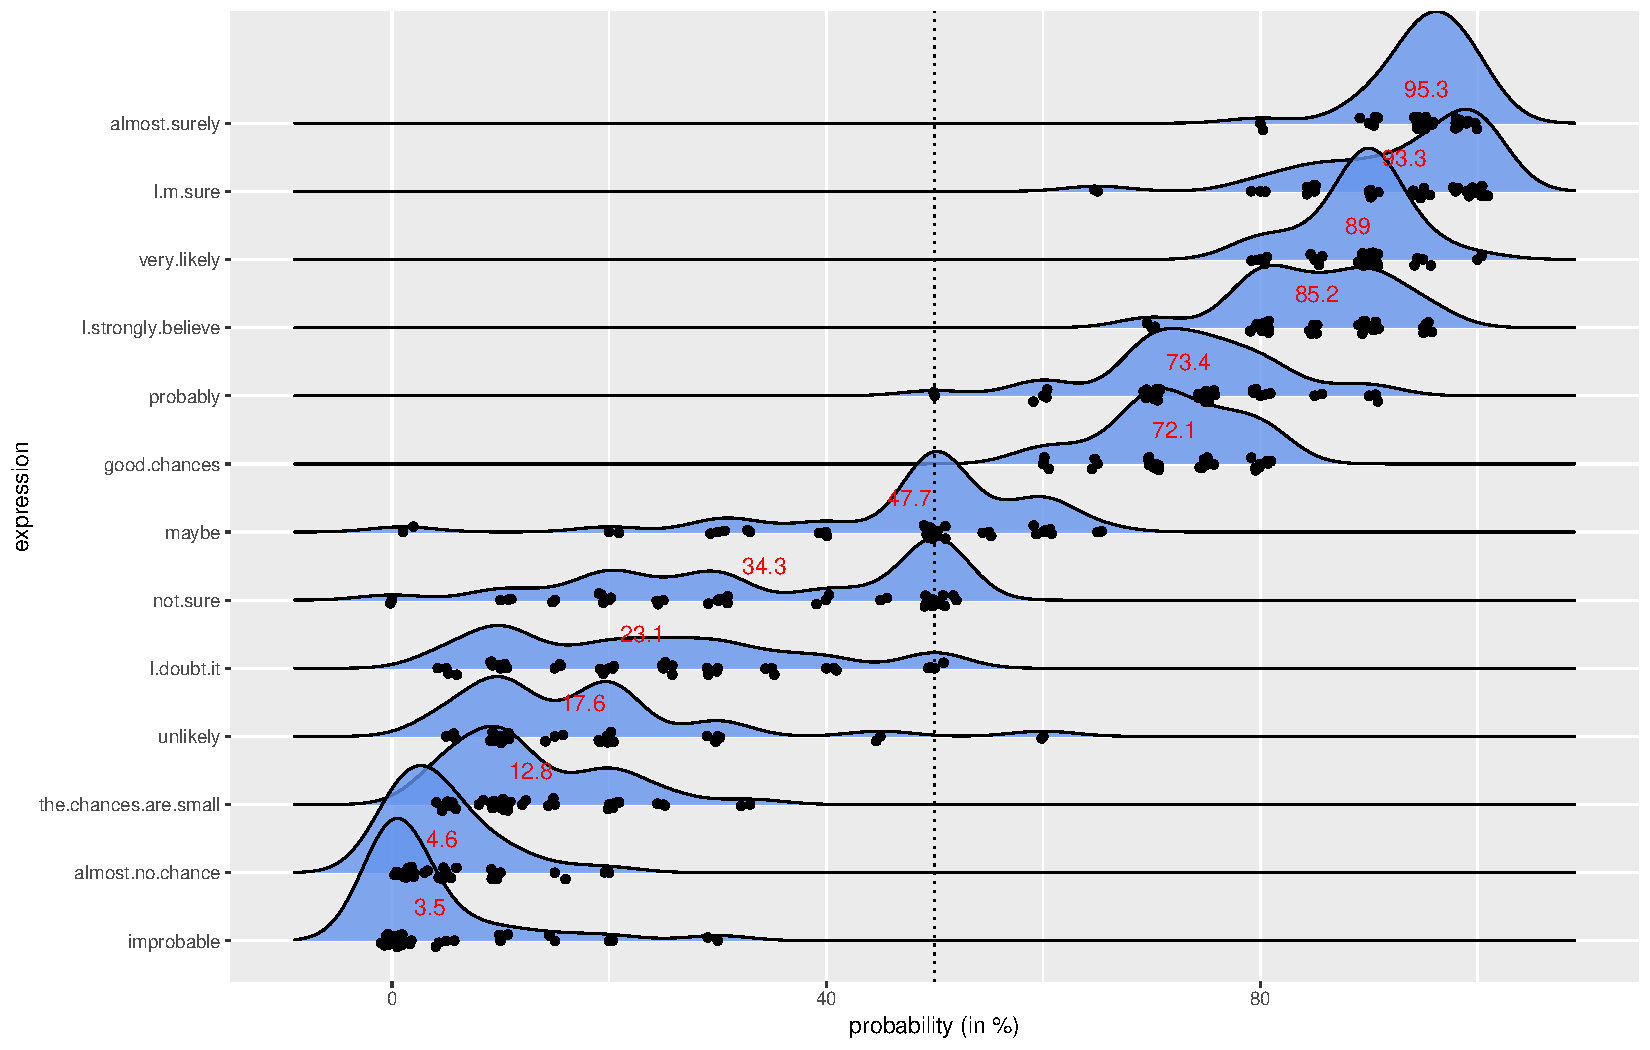
\includegraphics[width=0.95\linewidth]{../LectureAssets/L01/questionnaire}
\end{center}
\end{frame}

\begin{frame}{}
\centering
\bigskip
\bigskip
\smallskip
\begin{LARGE}
{\color{red} Q:} What will the temperature ($^\circ$C) be in Moscow at midnight?
\end{LARGE}
\end{frame}

\begin{frame}{Important observations}

\bigskip

\begin{itemize}\itemsep1.2em

\item Uncertainty is part of everyday life...

\item we've even developed natural language to express it!

\item However, natural language is imprecise, incoherent and lacks expressiveness...

\item which makes it useless for serious quantitative work.

\end{itemize}

\bigskip

Conclusion: \textbf{We need to agree on a more formal language for expressing uncertainty!}

\bigskip

\end{frame}


\begin{frame}{Formal definition of probability}

\begin{small}


\bigskip

Set of outcomes \textbf{$\Omega$} (set of all possible truths).

\smallskip

Set of events \textbf{$S$}  (all sets that we will assign probability to\footnote{The formalism used here is a $\sigma-$algebra.}).

\bigskip

A probability function $P$ a function $P:S \rightarrow [0,1]$ that satisfies the axioms of probability:

\begin{description}
\item[A1] $P(A) \geq 0, $ for all $A \in S$.
\item[A2] $P(\Omega) = 1.$
\item[A3] $P(A_1 \cup A_2 \cup A_3 \cup ...) = \sum_{i=1}^\infty P(A_i), \break \text{for any sequence of disjunct events}.$
\end{description}

\end{small}

\smallskip
\textbf{Why is probability defined like this and not something else?}


\end{frame}



\begin{frame}{Distributions}

\begin{columns}[c]
\column{3in}
\centering
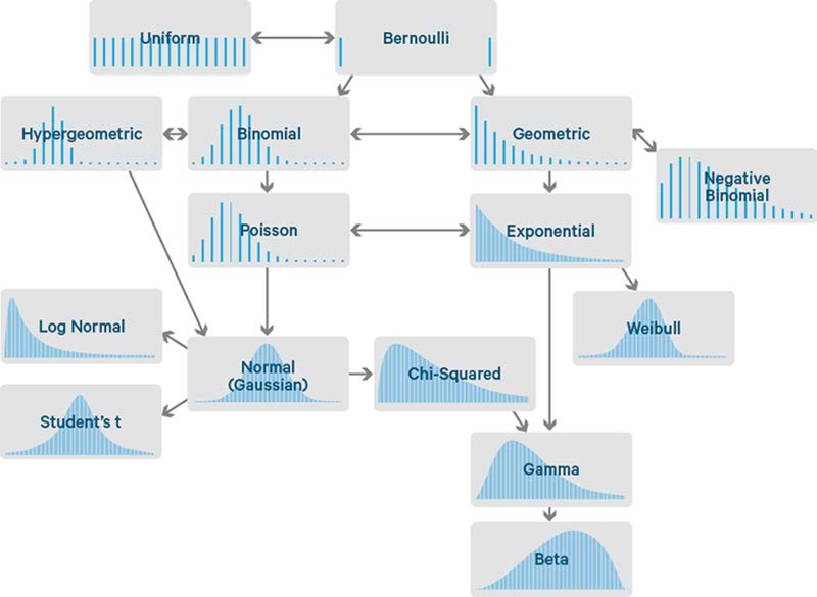
\includegraphics[width=0.90\linewidth]{../LectureAssets/L01/distributions}

\column{2in}
\begin{small}
\bigskip

Probability distributions are the elementary expressions of probabilistic thinking and
the basic building blocks of statistical models.

\bigskip

\bigskip

Distributions follow the axioms of probability and are therefore coherent and precise statements.

\end{small}

\end{columns}

\bigskip

\end{frame}


\begin{frame}{Bernoulli distribution}
\centering

$X \sim Bernoulli(p)$

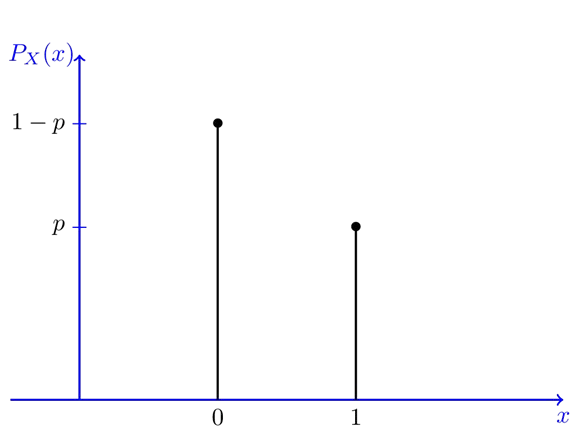
\includegraphics[width=0.50\linewidth]{../LectureAssets/L01/dist_C}

\bigskip
\pause
{\color{red} Q:} Will it rain in Moscow next Tuesday?
\bigskip
\end{frame}

\begin{frame}{Normal distribution}
\begin{center}

$X \sim N(\mu, \sigma^2)$

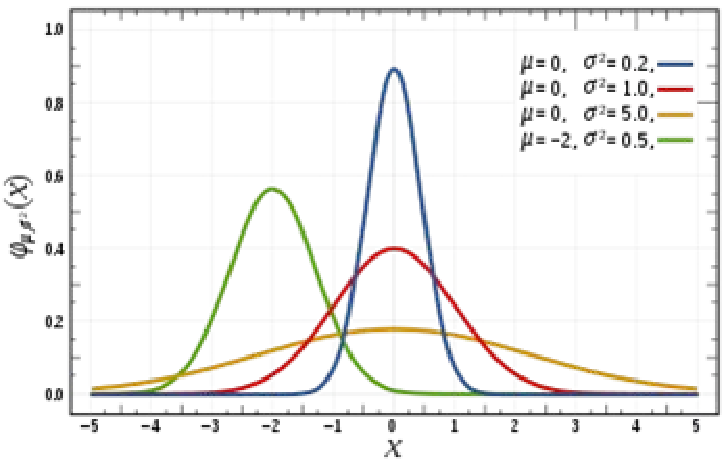
\includegraphics[width=0.50\linewidth]{../LectureAssets/L01/dist_N}

\bigskip
\pause
{\color{red} Q:} What will the temperature ($^\circ$C) be in Moscow at midnight?
\pause
\bigskip

{\color{red} Q:} What was the temperature ($^\circ$C) in Moscow exactly 50 years ago?
\bigskip
\pause
\end{center}
\begin{scriptsize}
What is the cause of uncertainty in the second case?

\vspace{-0.3cm}

What are some other common causes of uncertainty?
\end{scriptsize}

\end{frame}

\begin{frame}{Beta distribution}
\centering

$X \sim Beta(\alpha, \beta)$

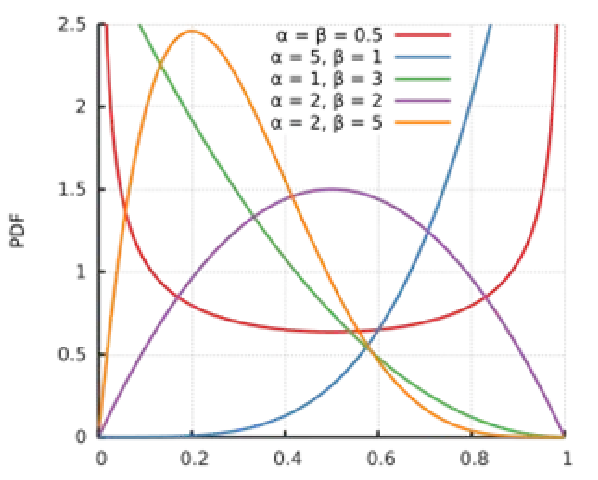
\includegraphics[width=0.50\linewidth]{../LectureAssets/L01/dist_B}

\bigskip

\bigskip
\end{frame}


\begin{frame}{Tricky questions}

Assume that these are independent tosses of a (possibly unfair) coin:

\begin{center}
\textbf{T  T  H  T  T  H  T  T  T  H} {\color{red}(?)}
\end{center}

\begin{small}
\bigskip
\begin{itemize}
\item {\color{red} Q1:} Will the 11th flip be heads or tails?\pause
\item {\color{red} Q2:} What is the coin‘s probability of landing heads?\pause
\item {\color{red} Q3:} Is this coin practically fair (is its probability between 49\% and 51\%)?
\end{itemize}
\end{small}
\bigskip
\end{frame}


\begin{frame}{Summary}

\begin{itemize}
\item Probability theory is a precise language for expressing uncertainty.
\item If we don‘t follow the rules of probability, others won‘t understand what we are saying! However, probability doesn't require us to be objective or even sensible.\footnote{For example, it's quite coherent to say that the world will end tomorrow with 0.99999 probability and there's a 0.00001 probability that it won't. But saying that there is a 0.99999 probability that it won't and 0.00002 probability that it will - that just doesn't make sense.}
\item And we find it natural to have probabilistic opinions about properties that are arguably not random.\footnote{This is inherently Bayesian!}
\end{itemize}
\end{frame}

\begin{frame}{Further reading}

See [HOFF:Ch02], [BDA:Ch01] for more on Bayesian probability. For a more thorough understanding of Bayesian probability, in particular, how axioms of probability and conditional probability follow from rationally avoiding being a sure loser in a betting game, see [POU:Ch01].

\bigskip

\begin{scriptsize}
\begin{itemize}
\item[BDA] Gelman, A., Carlin, J. B., Stern, H. S., Dunson, D. B., Vehtari, A., \& Rubin, D. B. (2013). Bayesian data analysis. CRC press.
\item[HOFF] Hoff, P. D. (2009). A first course in Bayesian statistical methods. New York: Springer.
\item [POU] Kadane, J. B. (2011). Principles of uncertainty. CRC Press.
\end{itemize}
\end{scriptsize}
\end{frame}

\end{document}
